\begin{problem}{Hypercube}{hypercube.in}{hypercube.out}{2 seconds}

% Author: Oleg Khristenko (idea), Roman Elizarov (text)

Consider a 4-hypercube also known as tesseract. A unit \emph{solid tesseract} is a 4D figure that 
is equal to the convex hull of 16 points with Cartesian coordinates $(\pm\frac{1}{2},\pm\frac{1}{2},\pm\frac{1}{2},\pm\frac{1}{2})$ ---
its vertices. It has 32 edges (1D), 24 square faces (2D), and 8 cubic 3-faces (3D) also known as \emph{cells}. 
We study hollow tesseracts and define a \emph{tesseract} as a boundary of a solid tesseract. Thus, a tesseract
is a connected union of 8 solid cubes (its cells) that intersect between each other at 
24 tesseract's square faces, 32 edges, and 16 vertices.

Let's cut a tesseract along 17 of its 24 faces, so that it still remains connected via 7 faces that were left intact. 
Unfold the tesseract into a 3D hyperplane by rotating its constituting cubes along the faces that were left intact until
all its cells lie in the same 3D hyperplane. The result is called a \emph{3-net} of a tesseract. This process is a
natural generalization of how a 3D cube is cut and unfolded onto a 2D plane to produce a 2-net of a cube that consists
of 6 squares. 

In this problem you are given a tree-like 8-polycube in 3D space also known as \emph{octocube}. 
An octocube is a collection of 8 unit cubical cells joined face-to-face.
More formally, intersection of each pair of cubical cells constituting an octocube is either empty, a point, a unit line (1D), or a unit square (2D). 
The given octocube is tree-like in the following sense. Consider an \emph{adjacency graph} of the octocube --- 
a graph with 8 vertices corresponding to its 8 cells. There is an edge in the adjacency graph between pairs of adjacent cells. 
Two cells of an octocube are called \emph{adjacent} when their intersection is a square. Cells that intersect at a point or a line are not considered adjacent.
An octocube is called \emph{tree-like} when its adjacency graph is a tree.

Your task is to determine whether the given tree-like octocube constitutes a 3-net of a tesseract. 
That is, whether this octocube being put onto a hyperplane in 4D space can be folded in 4D space along the squares of intersection
between its cells into a tesseract.

For example, look at the leftmost picture below. It shows a wire-frame of the tree-like octocube. Rotate cell
$GHLKG_1H_1L_1K_1$ around a plane $GHLK$ and cell $FGKJF_2G_2K_2J_2$ around a plane $FGKJ$ at angle 90 degrees in 4-th
dimension outside of the original hyperplane. As a result, point $G_1$ joins with $G_2$ and $K_1$ joins with $K_2$. The face
$GKK_2G_2$ is glued to face $GKK_1G_1$. The result is shown on the right. The 4-th dimension is orthographically projected onto 
the 3 shown in perspective.
The points that have moved out of the original hyperplane are marked with hollow dots.

\begin{figure}[h!]
\begin{minipage}[b]{0.5\textwidth}
\centering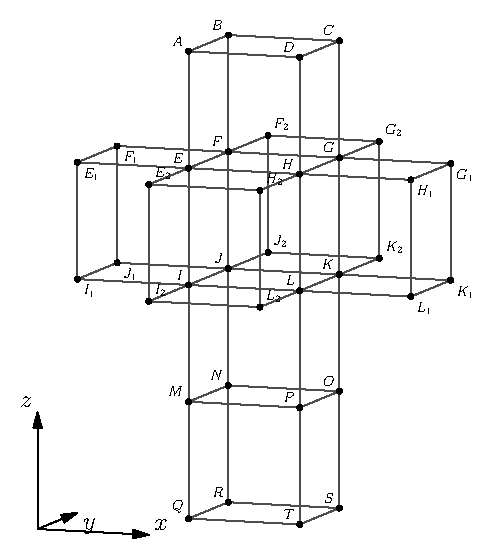
\includegraphics{pics/hypercube1.eps}
\end{minipage}%
\begin{minipage}[b]{0.5\textwidth}
\centering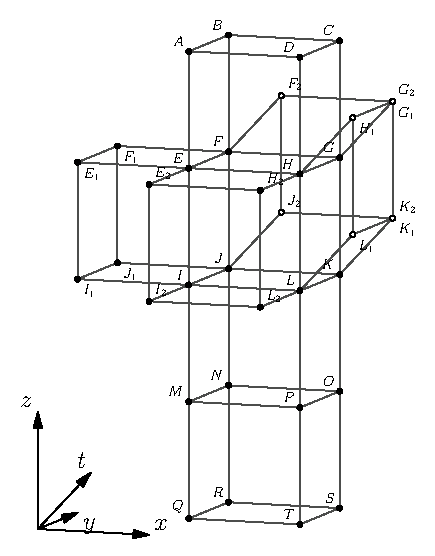
\includegraphics{pics/hypercube2.eps}
\end{minipage}%
\end{figure}

Rotate $EFJIE_1F_1J_1I_1$ around $EFJI$ and $EHLIE_2H_2L_2I_2$ around $EHLI$. The result is shown
on the following picture on the left. The remaining steps are as follows.
Rotate $MNOPQRST$ around $MNOP$, then
rotate both $MNOPQRST$ and $IJKLMNOP$ around $IJKL$ and rotate $ABCDEFGH$ around $EFGH$. The last step is to 
glue all faces that meet together to get a tesseract that is shown on the right. 

\begin{figure}[h!]
\begin{minipage}[b]{0.5\textwidth}
\centering\includegraphics{pics/hypercube3.eps}
\end{minipage}%
\begin{minipage}[b]{0.5\textwidth}
\centering\includegraphics{pics/hypercube4.eps}
\end{minipage}%
\end{figure}

\InputFile

The first line of the input file contains there integers $m$, $n$, $k$ --- 
the width, the depth, and the height of the box that contains the given octocube
($1 \le m, n, k \le 8$). The following $k$ groups of lines describe rectangular slices of the box from top to bottom. 
Each slice is described by $n$ rows with $m$ characters each. The characters on a line are either `\texttt{.}', 
denoting an empty space, or `\texttt{x}', denoting a unit cube.
The input file is guaranteed to describe a tree-like octocube.  

\OutputFile

Write to the output file a single word ``Yes'' if the given octocube can be folded into a tesseract 
or ``No'' otherwise.

\Example

\begin{example}
\exmp{
3 3 4
...
.x.
...
.x.
xxx
.x.
...
.x.
...
...
.x.
...
}{
Yes
}%
\exmp{
8 1 1
xxxxxxxx
}{
No
}%
\end{example}

\end{problem}
